\documentclass{beamer}
\usepackage{listings}
\usepackage[utf8]{inputenc} % special characters, my name, etc.
\usepackage{pslatex}	% postscript fonts
\usepackage{color}
\usetheme[nat,colourful]{Frederiksberg}

\lstset{language=C,
                basicstyle=\ttfamily,
                keywordstyle=\color{blue}\ttfamily,
                stringstyle=\color{red}\ttfamily,
                commentstyle=\color{green}\ttfamily,
                morecomment=[l][\color{magenta}]{\#}
}

\lstdefinestyle{customc}{
  belowcaptionskip=1\baselineskip,
  breaklines=true,
  frame=L,
  xleftmargin=\parindent,
  language=C,
  showstringspaces=false,
  basicstyle=\footnotesize\ttfamily,
  keywordstyle=\bfseries\color{green!40!black},
  commentstyle=\itshape\color{purple!40!black},
  identifierstyle=\color{blue},
  stringstyle=\color{orange},
}
\definecolor{codegreen}{rgb}{0,0.6,0}
\definecolor{codegray}{rgb}{0.5,0.5,0.5}
\definecolor{codepurple}{rgb}{0.58,0,0.82}
\definecolor{backcolour}{rgb}{0.95,0.95,0.92}

\lstdefinestyle{mystyle}{
    backgroundcolor=\color{backcolour},
    commentstyle=\color{codegreen},
    keywordstyle=\color{magenta},
    numberstyle=\tiny\color{codegray},
    stringstyle=\color{codepurple},
    basicstyle=\footnotesize,
    breakatwhitespace=false,
    breaklines=true,
    captionpos=b,
    keepspaces=true,
    numbers=left,
    numbersep=5pt,
    showspaces=false,
    showstringspaces=false,
    showtabs=false,
    tabsize=2
}

\lstset{style=mystyle}
%\lstset{escapechar=@,style=customc}


\title{The study of MIPS32 processor simulation}
\subtitle{Presentation}
\author{Jan Mezník,\\ pzj895@alumni.ku.dk}
\institute{Copenhagen University}
\date{\today}



\begin{document}

% Frontpage
\frame[plain]{\titlepage}



\begin{frame}
	\frametitle{Problem statement}
	\textit{Is it possible to implement a pipelined MIPS simulator, to fully
		support the current version of KUDOS?}\\
\end{frame}

\begin{frame}
	\frametitle{Learning objectives}

	\begin{itemize}
		\item Gain deeper understanding of the MIPS32 architecture

		\item How the CPU communicates with the IO devices

		\item Discover how operating systems interact with the CPU

		\item Learn the differences compared to other architectures

	\end{itemize}
\end{frame}

\begin{frame}
	\frametitle{Problem Analysis}
	KUDOS is based on the BUENOS operating system, originally developed at
	Aalto University, Finland.

\begin{block}{Requirements}
	\begin{itemize}
		\item Translation Lookaside Buffer
		\item Memory Management Unit
		\item I/O devices
		\item Pipeline (for our project)
	\end{itemize}
\end{block}
\begin{block}{Optional}
	\begin{itemize}
		\item SMP (multicore)
		\item Caches
	\end{itemize}
\end{block}
\end{frame}


\begin{frame}
	\frametitle{Implementation}
	\begin{center}
	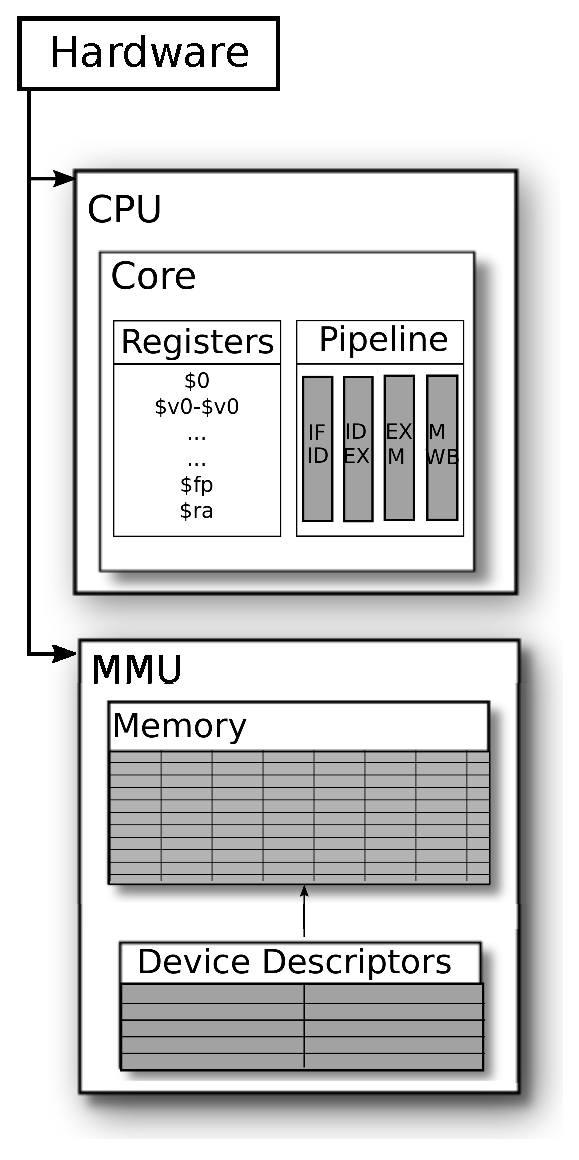
\includegraphics[scale=0.35]{../pipeline/structure_layout.eps}
	\end{center}
\end{frame}

\begin{frame}[fragile]
\frametitle{Pipeline}
\begin{columns}
\begin{column}{0.5\textwidth}

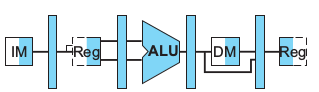
\includegraphics[scale=0.4]{simple_cpu.png}

\begin{verbatim}
void tick() {
   interpret_wb(...);
   interpret_mem(...);
   interpret_ex(...);
   interpret_id(...);
   interpret_if(...);
   forwarding_unit(...);
}
\end{verbatim}
\end{column}

\begin{column}{0.5\textwidth}

\begin{lstlisting}
struct reg_ex_mem {
	bool c_reg_write;
	bool c_branch;
	bool c_mem_read;
	bool c_mem_write;
	bool c_mem_to_reg;

	uint32_t eff_addr;
	uint32_t alu_res;

	uint32_t rt_value;
	uint8_t  reg_dst;
	uint32_t next_pc;
	uint32_t inst;
	exception_t exception;
};
\end{lstlisting}


\end{column}
\end{columns}
\end{frame}

\begin{frame}
\frametitle{Challenges with the Pipeline}

\begin{figure}
	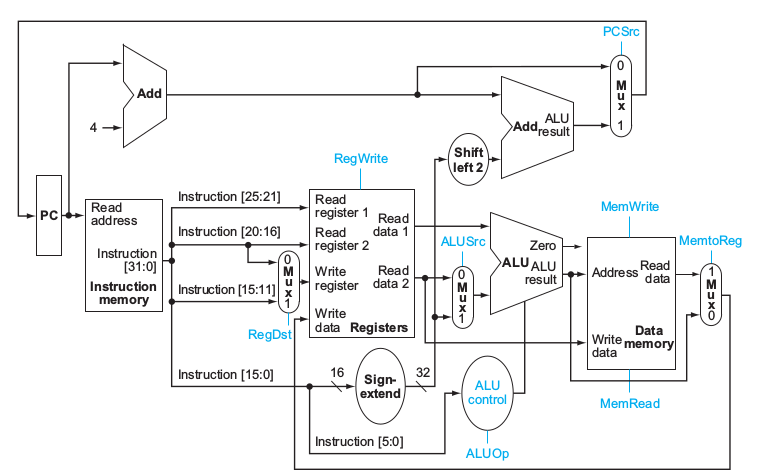
\includegraphics[scale=0.23]{cpu.png}
	\caption{Borrowed from COD5.}
\end{figure}

\begin{block}{Additions}
\begin{itemize}
	\item "New" instructions: \texttt{SH, SB, SWR, SWL, MFC0, etc.}
	\pause
	\item Interrupts from IO devices
	\pause
	\item Instructions with multiple side-effects: \texttt{SC, LL, ERET}
\end{itemize}
\end{block}
\end{frame}



\begin{frame}
\begin{center}
DEMO
\end{center}
\end{frame}


\begin{frame}
\frametitle{Improvements}
	\begin{itemize}
		\item Better IO handling (better device descriptors)
		\item Hotplug devices
		\item GNU Debugger integration
		\item Breakpoints
		\item Inspect and modify memory
		\item Backstepping
	\end{itemize}
\end{frame}


\begin{frame}
\begin{center}
Conclusion
\end{center}

\end{frame}

\end{document}
